%%%%%%%%%%%%%%%%%%%%%%%%%%%%%%%%%%%%%%%%%%%%%%%%%%%%%%%%%%%%%%%%%%%%%%%%%%%%%%%%%%%%%%%%
\section{Structure factor of a random flight model} \hspace{1pt}
\cite{Schweins2004,Burchard1970,Giehm2010}
\begin{align}
S_N(QD)&=
     \frac{2}{1-\frac{\sin⁡(QD)}{QD} )}-1-\frac{2\left[1-\left[\frac{\sin⁡(QD)}{QD}\right]^N \right]}{N\left[1-\frac{\sin⁡(QD)}{QD}\right]^2}   \frac{\sin⁡(QD)}{QD}
\end{align}
The formula above is only defined for the whole real space for integer values of $N$. For non integer values $n$ a linear interpolation between $[n]$ and $[n]+1$ is taken, where $[n]$ is the largest integer smaller or equal to $n$. With $w=n-[n]$ we get
\begin{align}
S_N(QD)&= (1-w)S_{[n]} + wS_{[n]+1}
\end{align}

%%%%%%%%%%%%%%%%%%%%%%%%%%%%%%%%%%%%%%%%%%%%%%%%%%%%%%%%%%%%%%%%%%%%%%%%%%%%%%%%%%%%%%%%
\section{ordered particle systems} \hspace{1pt}
\label{sec:ops}
This plugin contains the structure factor of ordered mesoscopic materials in case the domains are random orientated like in powder diffraction as described in \cite{Forster2005}. For oriented domains the scattering pattern is not anymore radial symmetric and depends both on the direction and modulus of the scattering vector. For this case the structure factor are taken from  \cite{Forster2011}. This plugin tries to re-implement the functions which are originally supplied by the software package \texttt{scatter} described in \cite{Forster2010}. The software package \texttt{scatter} is specialised on calculating and fitting ordered structures and has much more options and better GUI for this kind of studies. In both case the structure factor is approximated in the decoupling approach (\cite{Kotlarchyk1983}) as defined in \ref{sec:SQdecoupling} or in eq.\ \ref{Mittel} of section \ref{sec:decouplingGF}

In case of random oriented domains of three dimensional ordered particle systems the decoupling approach is implemented as
\begin{align}
I(Q) &= \langle\overline{F^2(Q)}\rangle_{or} + \langle\overline{F(Q)}\rangle_{or}^2 (S(Q)-1)
\end{align}
The overline symbol denotes the average over a particle size distribution and the brackets $\langle\rangle_{or}$ for the orientational average. In the above case it is assumed that the position of the scatterer is independent
of their size and orientation. For small size distributions and only small deviations from spherical symmetry of the scatterer the decoupling approximation works quite well.
For two and one dimensional ordered particle systems the particles can be very anisotropic, i.e.  very long cylindrical in case of 2D ordering and thin planar objects in case of 1D ordering. For this very anisotropic shaped particles the scattering amplitude and scattering intensity can be written as a product \ref{sec:very_anisotropic_particles} in terms of a cross section term for the short dimension $L_\mathrm{short}$ and a shape factor for the long dimension $L_\mathrm{long}$ as well as there averages
\begin{subequations}
\begin{align}
F(Q,L_\mathrm{short},L_\mathrm{long}) &= F_\mathrm{cs}(Q,L_\mathrm{short}) F'(Q,L_\mathrm{long}) \\
\langle\overline{F^2(Q,L_\mathrm{short},L_\mathrm{long})}\rangle_{or} &= \langle\overline{F^2_\mathrm{cs}(Q,L_\mathrm{short})}\rangle_{or} \langle\overline{F'^2(Q,L_\mathrm{long})}\rangle_{or} \\
\langle\overline{F(Q,L_\mathrm{short},L_\mathrm{long})}\rangle_{or}^2 &= \langle\overline{F_\mathrm{cs}(Q,L_\mathrm{short})}\rangle_{or}^2 \langle\overline{F'(Q,L_\mathrm{long})}\rangle_{or}^2
\end{align}
\end{subequations}

In case of one (multi-lamellar structures) as well as of two dimensional (ordering of structures on a planar surface) ordered particles strongly anisotropic particles are often ordered along their short dimension, i.e. cylindrical pillar have their cylindrical axis often perpendicular to the ordering plane or in case of lamellar structures ordering happens always in the direction of the normal of the planar scattering objects.
The averages, which needs to be performed in the decoupling approximation are
\begin{subequations}
\begin{align}
\label{eq:DecouplingPlusLattice}
I(\mathbf{Q}) &= \langle\langle\overline{F^2(\mathbf{Q})}\rangle_{i}\rangle_{d} + \langle\langle\overline{F(\mathbf{Q})}\rangle_{i}^2 (S(\mathbf{Q})-1)\rangle_{d} \\
&= \langle\langle\overline{F^2(\mathbf{Q})}\rangle_{i}\rangle_{d} + \langle\langle\overline{F(\mathbf{Q})}\rangle_{i}^2 (Z(\mathbf{Q})-1) G(\mathbf{Q})\rangle_{d}
\end{align}
\end{subequations}
with
\begin{align}
S(\mathbf{Q}) &= (Z(\mathbf{Q})-1) G(\mathbf{Q}) + 1
\end{align}
In the last equation the structure factor $S(\mathbf{Q})$ has been expressed in terms of the lattice factor function $Z(\mathbf{Q})$ and the Debye-Waller factor $G(\mathbf(Q))$. The term $Z(\mathbf{Q})G(\mathbf{Q})$ describes the decay of the Bragg peaks due to displacement and $1-G(\mathbf{Q})$ the concomitant increase of diffuse scattering. For a perfect lattice $G(\mathbf(Q))=1$.
The orientation averages is done here slightly different than in the paper from \cite{Forster2011}. The orientational averaging of the scatterer within the domain are denoted by $\langle\ldots\rangle_{i}$ and the orientation averaging of the whole domains by $\langle\ldots\rangle_{d}$
In the appendix of \cite{Forster2011} it is discussed under which conditions the orientation distribution over the structure factor and form factor can be factorized. If the orientation distribution of the scatterer in a domain is significant larger than the orientation distribution of the domains the averages can be factorized $\langle\left(\langle\ldots\rangle_{i}\right)^2\ldots\rangle_{d}\simeq\left(\langle\ldots\rangle_{i}\right)^2\langle \ldots\rangle_d$ and one obtains
\begin{subequations}
\begin{align}
I(\mathbf{Q}) &=  \langle\overline{F^2(\mathbf{Q})}\rangle_{i} + \langle\langle\overline{F(\mathbf{Q})}\rangle_{i}^2 (S(\mathbf{Q})-1)\rangle_{d} \\
&\simeq\langle\overline{F^2(\mathbf{Q})}\rangle_{i} + \langle\overline{F(\mathbf{Q})}\rangle_{i}^2 \langle(Z(\mathbf{Q})-1) G(\mathbf{Q})\rangle_{d}
\end{align}
\end{subequations}
The formula above is different to the one given in \cite{Forster2011}, where the orientational averaging is done after squaring the size average of the scattering amplitude $\langle\overline{F(\mathbf{Q})}^2\rangle_{or}$ instead of doing the orientation averaging first $\langle\overline{F(\mathbf{Q})}\rangle_{or}^2$.

However, in case of a powder signal, where the orientation distribution within a domain is small and the domains are random oriented. Also the structures can be very anisotropic in two or one dimensional ordered structures and the periodicity is in most cases perpendicular to the long dimension of the scattering object.

\subsection{Domains of ordered particle systems isotropically oriented}
\label{subsec:iso_ops}
~\newline

For random oriented domains of ordered particle systems the structure factor can be written as
\begin{align}
S(Q) &= \left(Z_0(Q)-1\right) G(Q) + 1
\end{align}
$Z_0(Q)$ is the lattice factor got an ideal undistorted lattice and $G(Q)$ the Debye-Waller factor. The lattice factor expressed with Miller indices reads as
\begin{align}
Z_0(Q) &= \frac{\left(2\pi\right)^{d-1}}{n v_d \Omega_d Q^{d-1}} \sum_{\{hkl\}} m_{hkl} f^2_{hkl} L_{hkl}(Q-Q_{hkl})
\end{align}
where $n$ is the number of particles per unit cell, $f_{hkl}$ is the symmetry factor taking into account extinction rules, $v_d$ is the volume ($d=3$), surface ($d=2$), or long-period ($d=1$) of the $d$-dimensional unit cell, $\Omega_d$ is the $d$-dimensional solid angle,  $L_{hkl}(Q-Q_{hkl})$ is a normalised peak-shape function, and $m_{hkl}$ is the multiplicity. If the sum is done over all reflections $\{hkl\}$, i.e. $\sum_{\{hkl\}}=\sum_{h=-\infty}^{\infty}\sum_{k=-\infty}^{\infty}\sum_{l=-\infty}^{\infty}$, one automatically accounts for multiplicity but one the costs for summing over all combinations of $\{hkl\}$. For the normalized peak shape function $L_{hkl}(x)$ the user can choose between Lorentzian, Gaussian, and Pearson VII peak shape
\begin{align}
L_{hkl}(x) &=
\begin{cases}
 \frac{2}{\pi\delta} \exp\left(-4\frac{x^2}{\pi\delta}\right)& \mbox{for Gaussian} \\
 \frac{\delta}{2\pi}\frac{1}{x^2+\left(\frac{\delta}{2}\right)^2}& \mbox{for Lorentzian} \\
 \frac{\left(1+\mathrm{B}^2\left(\nu-\frac12,\frac12\right)\left(\frac{x}{\delta}\right)^2\right)^{-\nu}}{\delta}& \mbox{for Pearson VII}
\end{cases}
\end{align}

To describe the diffraction pattern one has to define the unit cell of the ordered structure and the position of the particles with in the unit cell. The unit cell can be specified totally by six scalar quantities, which are called the unit cell dimensions or lattice parameters. These are (see also Fig.\ \ref{fig:UnitCellDimensions}:
$$ a,b,c,\alpha,\beta,\gamma $$
The first three parameters ($a$, $b$ and $c$) represent the lengths of the unit cell edges,
and the last three ($\alpha$,$\beta$ and $\gamma$) represent the angles between them. By convention, $\alpha$ is the angle between $b$ and $c$, $\beta$ is the angle between $a$ and $c$, and $\gamma$ is the angle between $a$ and $b$.
\begin{figure}[htb]
\begin{center}
\includegraphics[width=0.5\textwidth]{../images/structure_factor/OrderedParticleSystems/UnitCellParameters.png}
\end{center}
\caption{Unit cell in three dimensions. } \label{fig:UnitCellDimensions}
\end{figure}

If we assume that the vectors $\mathbf{a}$ and $\mathbf{b}$ are in the $x$-$y$ plane and $\mathbf{a} \| \mathbf{e}_x$ we can write the vector of the unit cell as
\begin{align}
\label{eq:direct_lattice_vector}
\mathbf{a} = a \spvec{1;0;0}
\qquad
\mathbf{b} = b \spvec{\cos \gamma;\sin \gamma;0}
\qquad
\mathbf{c} = c \spvec{\cos\beta;\frac{\cos\alpha-\cos\beta \cos\gamma}{\sin\gamma};\sqrt{1-\cos^2\beta-\left(\frac{\cos\alpha-\cos\beta \cos\gamma}{\sin\gamma}\right)^2}}
\end{align}
Next to the direct lattice with $\mathbf{a}$, $\mathbf{b}$, and $\mathbf{c}$ be the elementary
translations in a three-dimensional lattice a second lattice, reciprocal to the direct lattice, is defined by three elementary translations $\mathbf{a}^\star$, $\mathbf{b}^\star$ and $\mathbf{c}^\star$
\begin{align}
\label{eq:reciprocal_lattice_vector}
\mathbf{a}^\star = \frac{\mathbf{b}\times\mathbf{c}}{\mathbf{a}\cdot (\mathbf{b}\times\mathbf{c})}
\qquad
\mathbf{b}^\star = \frac{\mathbf{c}\times\mathbf{a}}{\mathbf{a}\cdot (\mathbf{b}\times\mathbf{c})}
\qquad
\mathbf{c}^\star = \frac{\mathbf{a}\times\mathbf{b}}{\mathbf{a}\cdot (\mathbf{b}\times\mathbf{c})}
\end{align}
For the scalar product between the direct and reciprocal lattice the following conditions holds:
\begin{subequations}
\begin{align}
\mathbf{a}\cdot\mathbf{a}^\star&=1 & \mathbf{a}\cdot\mathbf{b}^\star&=0 & \mathbf{a}\cdot\mathbf{c}^\star&=0 \\
\mathbf{b}\cdot\mathbf{a}^\star&=0 & \mathbf{b}\cdot\mathbf{b}^\star&=1 & \mathbf{b}\cdot\mathbf{c}^\star&=0 \\
\mathbf{c}\cdot\mathbf{a}^\star&=0 & \mathbf{c}\cdot\mathbf{b}^\star&=0 & \mathbf{c}\cdot\mathbf{c}^\star&=1
\end{align}
\end{subequations}
For a two dimensional periodic lattice with the direct lattice vectors $\mathbf{a}, \mathbf{b}$ and reciprocal lattice vector $\mathbf{a}^\star, \mathbf{b}^\star$ the orthogonal relations above also hold and by using eq.\ \ref{eq:reciprocal_lattice_vector} with $\mathbf{c}=\spvec{0,0,1}^T$ ($c=1,\alpha=\beta=\pi/2$) one can calculate them in the same way.
\begin{subequations}
\begin{align}
\label{eq:2D_lattice_vector}
\mathbf{a} &= a \spvec{1;0;0}  & \mathbf{b} &= b \spvec{\cos \gamma;\sin \gamma;0} \\
\mathbf{a}^\star &= \frac{1}{a} \spvec{1;-\frac{\cos\gamma}{\sin\gamma};0} &  \mathbf{b}^\star &= \frac{1}{b} \spvec{0;\frac{1}{\sin \gamma};0}
\end{align}
\end{subequations}
Last but not least, for a one dimensional lattice $\mathbf{a}=\spvec{a,0,0}^T$ the reciprocal lattice vector is simply $\mathbf{a}^\star=\frac1a\spvec{1,0,0}^T$.

Diffraction peaks can occur at integer multiples, called Miller indices $(hkl)$, of the reciprocal lattice
\begin{subequations}
\begin{align}
\mathbf{Q}_{hkl}^{3D} &= 2\pi\left( h\mathbf{a}^\star+k\mathbf{b}^\star+l\mathbf{c}^\star \right) \\
\mathbf{Q}_{hk}^{2D} &= 2\pi\left( h\mathbf{a}^\star+k\mathbf{b}^\star\right) \\
\mathbf{Q}_{h}^{1D} &= 2\pi h\mathbf{a}^\star
\end{align}
\end{subequations}
Due to the symmetry of the unit cell certain $(hkl)$ reflections might be forbidden. This is described by the structure factor of the unit cell $f_{hkl}$. The structure factor depends next to the Miller indices also from the type and position of the scattering objects within the unit cell. The position $\mathbf{R}_i(u,v,w)$ of the $i^\mathrm{th}$ scatterer with the scattering amplitude $F_i(\mathbf{Q})$ in the unit cell is normally given in terms of the direct lattice vectors $\mathbf{a}$, $\mathbf{b}$, and $\mathbf{c}$
\begin{align}
\mathbf{R}_i(u_i,v_i,w_i) = u_i \mathbf{a} + v_i\mathbf{b} +w_i\mathbf{c}
\end{align}
The scattering amplitude of the unit cell $f_{hkl}$ is than given by
\begin{subequations}
\begin{align}
f_{hkl} (\mathbf{Q}_{hkl}) &= \sum_{i=1}^N F_i(\mathbf{Q}_{hkl}) \exp\left( -\imath \mathbf{Q}_{hkl} \mathbf{R}_i\right) \\
                          &= \sum_{i=1}^N F_i(\mathbf{Q}_{hkl}) \exp\left( -\imath 2\pi \left(hu_i+kv_i+lw_i\right)\right) \\
&=  \sum_{i=1}^N F_i(\mathbf{Q}_{hkl}) \left[ \cos\left( 2\pi \left(hu_i+kv_i+lw_i\right)\right) \right. \nonumber \\
    & \qquad \qquad \qquad \qquad \left.- \imath \sin\left( 2\pi \left(hu_i+kv_i+lw_i\right)\right) \right] \\
    &= \sqrt{A^2+B^2} \exp(-\imath \arctan(\sfrac{A}{B}))
\end{align}
\end{subequations}
with
\begin{subequations}
\begin{align}
A &= \sum_{i=1}^N F_i(\mathbf{Q}_{hkl}) \cos\left( 2\pi \left(hu_i+kv_i+lw_i\right)\right) \\
B &= \sum_{i=1}^N F_i(\mathbf{Q}_{hkl}) \sin\left( 2\pi \left(hu_i+kv_i+lw_i\right)\right)
\end{align}
\end{subequations}
For a 2D and 1D lattice the scattering amplitude of the unit cell $f_{hk}$ and $f_h$ are calculated accordingly.
\begin{table}[htb]
  \centering
  \scriptsize
  \setlength\doublerulesep{0pt}
\begin{tabular}{|>{\columncolor[gray]{1.0}[0.8\tabcolsep][0.8\tabcolsep]} l%
                |>{\columncolor[gray]{1.0}[0.8\tabcolsep][0.8\tabcolsep]} c%
                |>{\columncolor[gray]{1.0}[0.8\tabcolsep][0.8\tabcolsep]} c%
                |>{\columncolor[gray]{1.0}[0.8\tabcolsep][0.8\tabcolsep]} c%
                |>{\columncolor[gray]{1.0}[0.8\tabcolsep][0.8\tabcolsep]} c|}
 \rowcolor[gray]{0.7}
 lattice & LAM &  SQ  &  HEX  & CREC \\
 \rowcolor[gray]{0.7}
 & & (P4/mm) & (P6/mm) & (cmm)  \\
  \hline\hline
 $n$ & 1 & 1 & 1 & 2 \\
 \rowcolor[gray]{0.95}
 $v_d$ & $a$ & $a^2$& $\sqrt{3}a^2/2$ & $ab$ \\
 $d$ & 1 & 2 & 2 & 2 \\
 \rowcolor[gray]{0.95}
 $f_{hkl}$ & $f_h=1$ & $f_{hk}=1$ & $f_{hk}=1$ & $f_{hk}=1$  \\
 $m_{hkl}$ & & & & \\
 \rowcolor[gray]{0.95}
 $\Omega_d$ & 1 & $2\pi$ & $2\pi$ & $2\pi$  \\
 $\overline{a}$ & $a$ & $a$ & $a$ & $\min\left\{a,b,\frac12\sqrt{a^2+b^2}\right\}$  \\
 \rowcolor[gray]{0.95}
 $Q_{hkl}$ & $ \frac{2\pi h}{a}$ & $\frac{2\pi\sqrt{h^2+k^2}}{a}$ & $\frac{4\pi\sqrt{h^2+hk+k^2}}{\sqrt{3}a}$ & $2\pi\sqrt{\frac{h^2}{a^2}+\frac{k^2}{b^2}}$ \\
\hline
\end{tabular}

\vspace{3mm}

\begin{tabular}{|>{\columncolor[gray]{1.0}[0.8\tabcolsep][0.8\tabcolsep]} l%
                |>{\columncolor[gray]{1.0}[0.8\tabcolsep][0.8\tabcolsep]} c%
                |>{\columncolor[gray]{1.0}[0.8\tabcolsep][0.8\tabcolsep]} c%
                |>{\columncolor[gray]{1.0}[0.8\tabcolsep][0.8\tabcolsep]} c%
                |>{\columncolor[gray]{1.0}[0.8\tabcolsep][0.8\tabcolsep]} c%
                |>{\columncolor[gray]{1.0}[0.8\tabcolsep][0.8\tabcolsep]} c|}
 \rowcolor[gray]{0.7}
 lattice &  BCT  &  FCC  & BCC & HCP & SC\\
 \rowcolor[gray]{0.7}
 &(I4/mmm)& (Fm3m) & (Im3m) & (P6/mmc) & (Pm3m) \\
  \hline\hline
 $n$ & 2 & 4 & 2 & 2 & 1\\
 $\mathbf{R}_i=\spvec{u_i;v_i;w_i}$ & $\spvec{0;0;0}$, $\spvec{\sfrac12;\sfrac12;\sfrac12}$ & $\spvec{0;0;0}$, $\spvec{\sfrac12;\sfrac12;0}$, $\spvec{\sfrac12;0;\sfrac12}$, $\spvec{0;\sfrac12;\sfrac12}$ & $\spvec{0;0;0}$, $\spvec{\sfrac12;\sfrac12;\sfrac12}$ & $\spvec{0;0;0}$, $\spvec{\sfrac23;\sfrac13;\sfrac12}$ & $\spvec{0;0;0}$\\
 \rowcolor[gray]{0.95}
 $v_d$ & $a^2 c$ & $a^3$ & $a^3$ & $\sqrt{2}a^3$ & $a^3$\\
 $d$ & 3 & 3 & 3 & 3 & 3\\
 \rowcolor[gray]{0.95}
 $ \abs{f_{hkl}}$ & $\scriptscriptstyle \abs{1+\cos(\pi(h+k+l))}$ &
    $\scriptscriptstyle \abs{\begin{array}{l@{}}  \scriptscriptstyle 1+\cos(\pi(h+k)) \\ \scriptscriptstyle +\cos(\pi(h+l)) \\ \scriptscriptstyle +\cos(\pi(k+l))\end{array}}$ &
    $\scriptscriptstyle \abs{1+\cos(\pi(h+k+l))}$ &
    $\scriptscriptstyle \abs{2\cos\left(\pi\left(\frac{h+2k}{3}+\frac{l}{2}\right)\right)}$ &
    $\scriptscriptstyle f_{hkl}=1$ \\
 $m_{hkl}$ & & & & & \\
 \rowcolor[gray]{0.95}
 $\Omega_d$ & $4\pi$ & $4\pi$ & $4\pi$ & $4\pi$ & $4\pi$ \\
 $\overline{a}$ & $\sqrt{2}a/2$ & $\sqrt{2}a/2$ & $\sqrt{3}a/2$ & $a$ & $a$ \\
 \rowcolor[gray]{0.95}
 $Q_{hkl}$ &  $\scriptscriptstyle 2\pi\sqrt{\frac{h^2+k^2}{a^2}+\frac{l^2}{c^2}}$ &
  $\scriptscriptstyle \frac{2\pi\sqrt{h^2+k^2+l^2}}{a}$ & $\scriptscriptstyle \frac{2\pi\sqrt{h^2+k^2+l^2}}{a}$ & $\scriptscriptstyle \frac{2\pi\sqrt{\frac43(h^2+hk+k^2)+\frac38 l^2}}{a}$ & $\scriptscriptstyle \frac{2\pi\sqrt{h^2+k^2+l^2}}{a}$\\
\hline
\end{tabular}

\vspace{3mm}
\caption{}
\label{tab:opoiso}
\end{table}


\subsection{Domains of ordered particle systems with preferred orientation}
\label{subsec:aniso_ops}
~\newline



\begin{figure}[htb]
\begin{center}
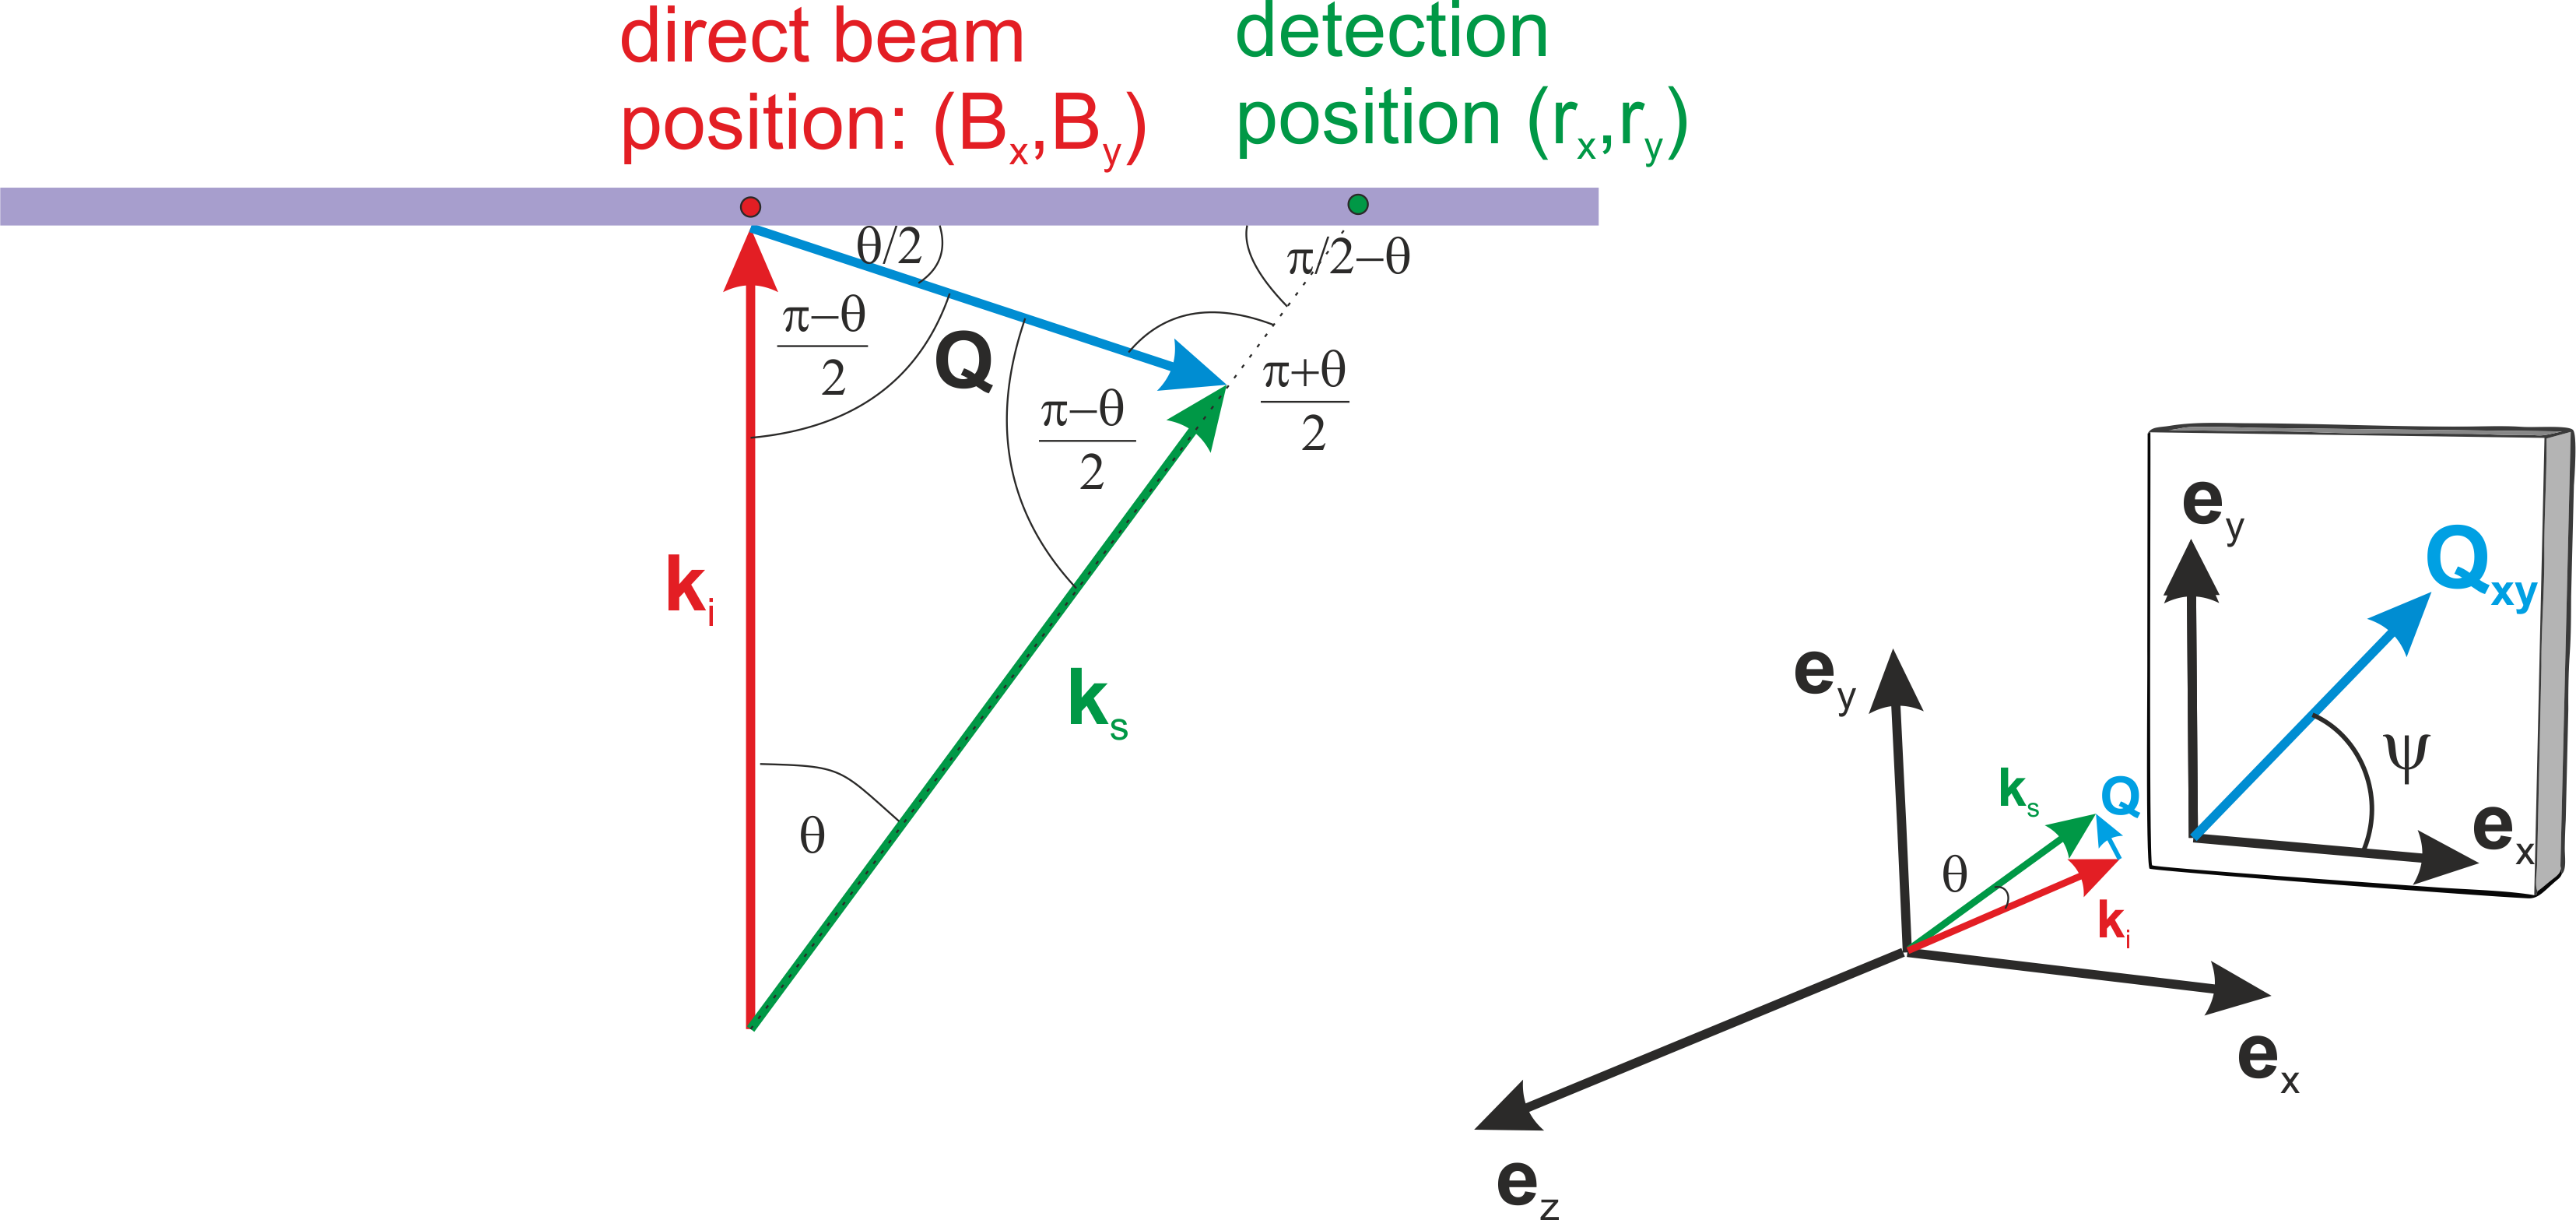
\includegraphics[width=0.85\textwidth]{osp_coord_system.png}
\end{center}
\caption{The scattering vector in polar coordinates coordination system with respect to a laboratory-fixed coordinate system based on the three orthogonal unit vectors ($\mathbf{e}_x$, $\mathbf{e}_y$, $\mathbf{e}_z$). They are arranged such that the x-direction coincides with the x-direction of the detector, and the y-direction coincides with the y-direction of the detector. The direction of the incoming neutron beam is chosen to be $-\mathbf{e}_z$. } \label{fig:opsCoordSys}
\end{figure}

\begin{align}
\mathbf{k}_i &=
    \left(
        \begin{array}{c}
                  k_{i,x} \\
                  k_{i,y} \\
                  k_{i,z}
        \end{array}
    \right)
    = \frac{2\pi}{\lambda}
    \left(
        \begin{array}{c}
                  0\\
                  0 \\
                  -1
        \end{array}
    \right) \\
\mathbf{k}_s &=
    \left(
        \begin{array}{c}
                  k_{i,x} \\
                  k_{i,y} \\
                  k_{i,z}
        \end{array}
    \right)
    = \frac{2\pi}{\lambda}
    \left(
        \begin{array}{c}
                  \cos(\psi) \sin(\theta)\\
                  \sin(\psi) \sin(\theta) \\
                  -\cos(\theta)
        \end{array}
    \right) \\
\mathbf{Q} &= \mathbf{k}_s - \mathbf{k}_i =
    \left(
        \begin{array}{c}
                  Q_{x} \\
                  Q_{y} \\
                  Q_{z}
        \end{array}
    \right)
    = \frac{2\pi}{\lambda}
    \left(
        \begin{array}{c}
                  \cos(\psi) \sin(\theta)\\
                  \sin(\psi) \sin(\theta) \\
                  1-\cos(\theta)
        \end{array}
    \right)
\end{align} 